\documentclass[10.5pt]{article}   %11 puntos

%Adapted from Adapted from UWA Engineering Final Year Project.


\usepackage[utf8]{inputenc}
\usepackage[x11names,dvipsnames,svgnames,table]{xcolor}

% general incantations
\usepackage[export]{adjustbox}
\usepackage{afterpage}

\usepackage{graphicx}
\usepackage{placeins}
\usepackage{pdfpages}
\usepackage{algorithm2e}
\usepackage{array}
\usepackage{booktabs}
\usepackage[most]{tcolorbox}
\usepackage{calligra}
\usepackage{caption}
\usepackage{datetime}
\usepackage{dirtytalk}
\usepackage{dsfont}
\usepackage{etex}
\usepackage{fancyhdr}
\usepackage{fix-cm}
\usepackage[T1]{fontenc}
\usepackage{textcomp,gensymb} %for \degree C symbol
\usepackage{graphicx}
\usepackage{lipsum}
\usepackage{listings}
\usepackage{transparent}
\usepackage[everyline=true,framemethod=tikz]{mdframed}
\usepackage{mparhack}
\usepackage{multicol}
\usepackage{multirow}
\usepackage{parskip}
\usepackage{lscape}
\usepackage{pdflscape}
\usepackage{pdfpages}
\usepackage{placeins}
\usepackage[document]{ragged2e}
\usepackage{rotating}
\usepackage{setspace}
\usepackage{subcaption}
\usepackage{threeparttable}
\usepackage[normalem]{ulem}
\usepackage{verbatim}
\usepackage{soul} %highlighting, strike through etc.

%Automated appendices
\usepackage[titletoc,title,header]{appendix} %advanced functionality

%language settings
\usepackage[utf8]{inputenc}
\usepackage{csquotes}

%page setup
%this where we adjust the binding offset, if relevant
\usepackage{geometry}
\geometry{left=2cm,right=2cm,top=2cm,bottom=2cm}
\usepackage{lastpage} % for page 1 of n footers

%cross referencing
\usepackage[hidelinks]{hyperref}
\usepackage{cleveref}

%maths stuff
\usepackage{amsmath}
\usepackage{mathtools}

\setcounter{secnumdepth}{5}

%lists
\usepackage{enumitem}

%working collaboratively
\usepackage[backgroundcolor=yellow]{todonotes}

% bibliography file using harvard
\usepackage[style=apa,citestyle=bwl-FU,backend=biber, sorting=nyt]{biblatex}
\bibliography{bibliography.bib} % with extension

%glossary for acronyms
\usepackage[acronym,nonumberlist,toc,section=subsection,numberedsection=nolabel]{glossaries} 
\makeglossaries

%line spacing
\linespread{1.6}


\usepackage{times}                      %Times New Roman
\usepackage{setspace}                   %Para espaciar
%\linespread{1.25}                      %Interlineado 1.5
%\singlespacing                          %Espaciado simple

\newcommand*\Heq{\ensuremath{\overset{\kern2pt LH }{=}}}
\newcommand{\Lagr}{\mathcal{L}}         %L (lagrangiano o fun de verosimilitud)
\newcommand{\indep}{\rotatebox[origin=c]{90}{$\models$}}
\newcommand{\R}{\mathbb{R}}             %Real numbers
\usepackage[utf8x]{inputenc}
%\usepackage{apacite}                    %Citas tipo apa
%\renewcommand{\thesubsection}{\thesection.\alph{subsection}}
%\usepackage{cite}
%\usepackage[left=2.5cm,right=2.5cm,top=2.5cm,bottom=2.5cm]{geometry} %Deberían ser 3 y 3 los left y right pero lo hago así para que entre mejor
%\usepackage[round]{natbib}              %Bibliografía
%\usepackage[utf8]{inputenc}
%\usepackage{amsmath}
\usepackage{mathtools}                  %Loads amsmath
\usepackage{amssymb}

\numberwithin{equation}{section}
\usepackage{hyperref}
\usepackage{color}   %May be necessary if you want to color links
 \hypersetup{
     colorlinks=false, %set true if you want colored links
     linktoc=all,     %set to all if you want both sections and sections linked
     linkcolor=blue,  %choose some color if you want links to stand out
 }
 \usepackage[spanish,es-tabla]{babel}
 \usepackage{graphicx}
 \usepackage{physics}
 %\usepackage[hidelinks]{hyperref}

\usepackage{amssymb}    %Para tener los check mark y cruces
\usepackage{pifont}     %Para tener los check mark y cruces
\newcommand{\cmark}{\ding{51}} %Para tener los check mark y cruces
\newcommand{\xmark}{\ding{55}}  %Para tener los check mark y cruces
\usepackage{float}

%Esto lo podés volar
% \usepackage{xcolor}                 %Night mode
% \pagecolor[rgb]{0,0,0} %black       %Night mode
% \color[rgb]{0.8,0.8,0.8} %grey      %Night mode

\title{Mapas y gráficos R}
\author{Matías Harari y Mariana Santi}
\date{2° trimestre 2021}
\setlength{\marginparwidth}{2cm}
\usepackage{setspace}
\spacing{1.2}
\usepackage{listings}
\usepackage{color}

\definecolor{dkgreen}{rgb}{0,0.6,0}
\definecolor{gray}{rgb}{0.5,0.5,0.5}
\definecolor{mauve}{rgb}{0.58,0,0.82}

\lstset{frame=tb,
  language=Java,
  aboveskip=3mm,
  belowskip=3mm,
  showstringspaces=false,
  columns=flexible,
  basicstyle={\small\ttfamily},
  numbers=none,
  numberstyle=\tiny\color{gray},
  keywordstyle=\color{blue},
  commentstyle=\color{dkgreen},
  stringstyle=\color{mauve},
  breaklines=true,
  breakatwhitespace=true,
  tabsize=3
}

\begin{document}
\renewcommand{\thesubsection}{\thesection.\alph{subsection}}

\thispagestyle{empty}
\setlength\headheight{0pt} 
\begin{center}

\begin{center}

\includegraphics[width=0.65\linewidth]{imgs/logoudesa.png}            
\end{center}	

        \vspace{0.2cm}
        {\scshape\LARGE Departamento de Economía \par}
        \vspace{0.2cm}
        {\scshape\Large Maestría en Economía\par}
        \vspace{0.4cm}

        {\Large\bfseries Herramientas computacionales - Gráficos en R y principios de Schwabish\par}
        
        \vspace{1cm}
        {\Large\itshape Matias Harari y Mariana Santi \par}


\vspace{1cm} 
\large
{2021}

\end{center}

\clearpage
\justify
\section*{Gráficos sobre resultados de elecciones electorales}
La Figura \ref{mylabel:fig1} incumple con los principios 1 y 2 de Schwabish ya que el formato puede ajustarse para que el mensaje sea más claro y contiene elementos visuales innecesarios. En primer lugar, el mapa especifica las coordenadas de latitud y longitud en los ejes, lo cual no aporta información relevante y vuelve más compleja la lectura. En segundo lugar, presenta colores estridentes que no resultan agradables a la vista. En tercer lugar, el título de la leyenda resulta innecesario ya que dicha información puede presentarse en el título. Por último, para simplificar la lectura de los datos, es conveniente colocar porcentajes en lugar de proporciones. En la Figura \ref{fig2} se muestra el mismo gráfico corrigiendo los errores comentados. Como se puede observar, el mensaje es más claro y la escala de colores, además de ser más agradable, refleja de mejor manera el mensaje ya que establece con el mismo color un tono más fuerte para los estados con mayor cantidad de votos en relación a su población y un tono más claro para el caso contrario. Esta opción resulta superadora ya que al tratarse de una sola variable, es más natural utilizar un único color.
\begin{figure}[H]
\centering
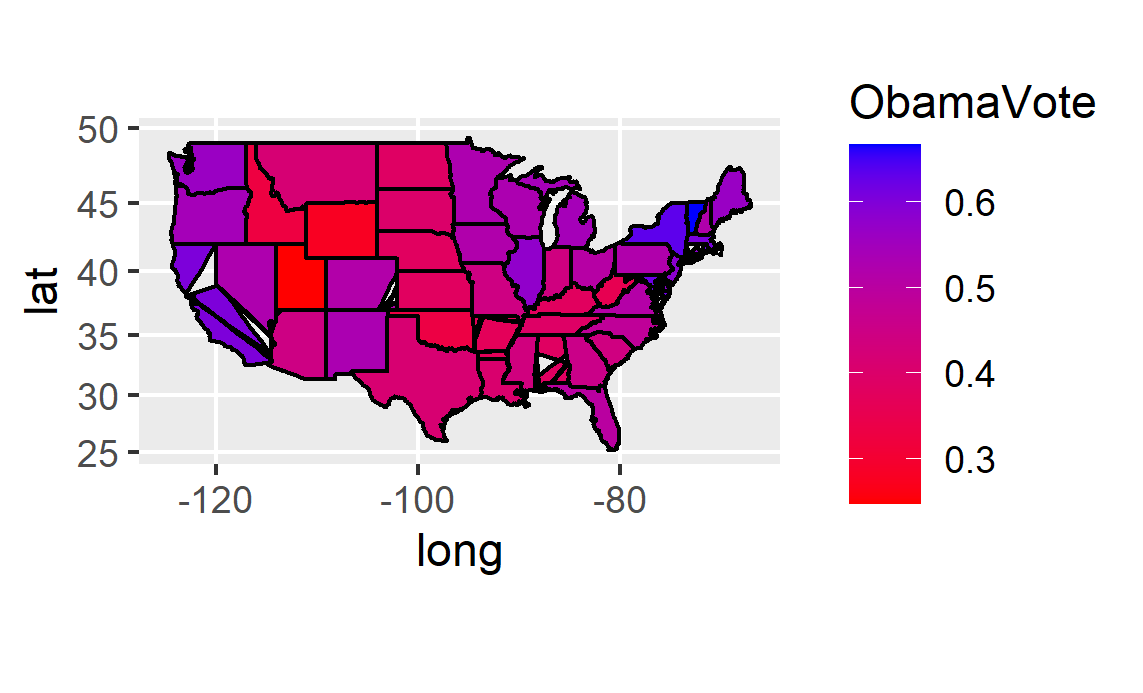
\includegraphics[scale=1.3]{imgs/Obamavote1.png}
\caption{Mapas sobre resultados de las elecciones de 2012 con errores}
    \label{mylabel:fig1}
\end{figure}
\begin{figure}[H]
\centering
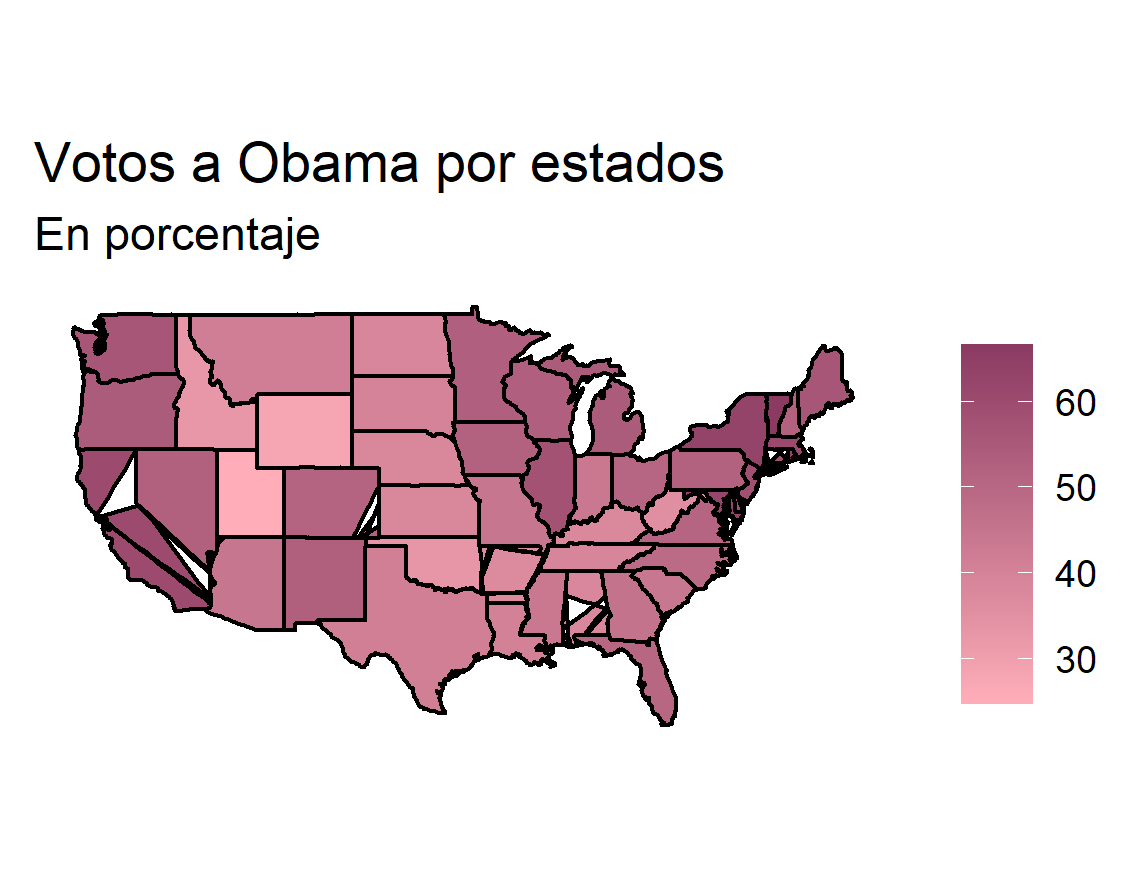
\includegraphics[scale=1]{imgs/Obamavote2.png}
\caption{Mapas sobre resultados de las elecciones de 2012 corregido}
    \label{fig2}
\end{figure}


\section*{Scatter plots con datos de préstamos}
La Figura \ref{fig3} también incumple con los principios 1 y 2. En primer lugar, los títulos de los ejes no son claros. Las bases de datos suelen contener nombres de variables reducidos y deben ser corregidos en los gráficos o se debe aclarar a qué refieren las abreviaciones en el documento. En segundo lugar, dado que el objetivo es observar la correlación entre los pagos recibidos y otras dos variables, resulta conveniente colocar a la primera variable en el eje $y$ para colocar sólo una vez el título y así evitar repetir información. En tercer lugar, los valores que indican los ejes deberían expresarse en otra unidad (en este caso, en miles) para simplificar la lectura. Por último, la leyenda podría incluirse en el título para evitar duplicar información. En la Figura \ref{fig4}, se corrigen dichos errores.
\begin{figure}[H]
\centering
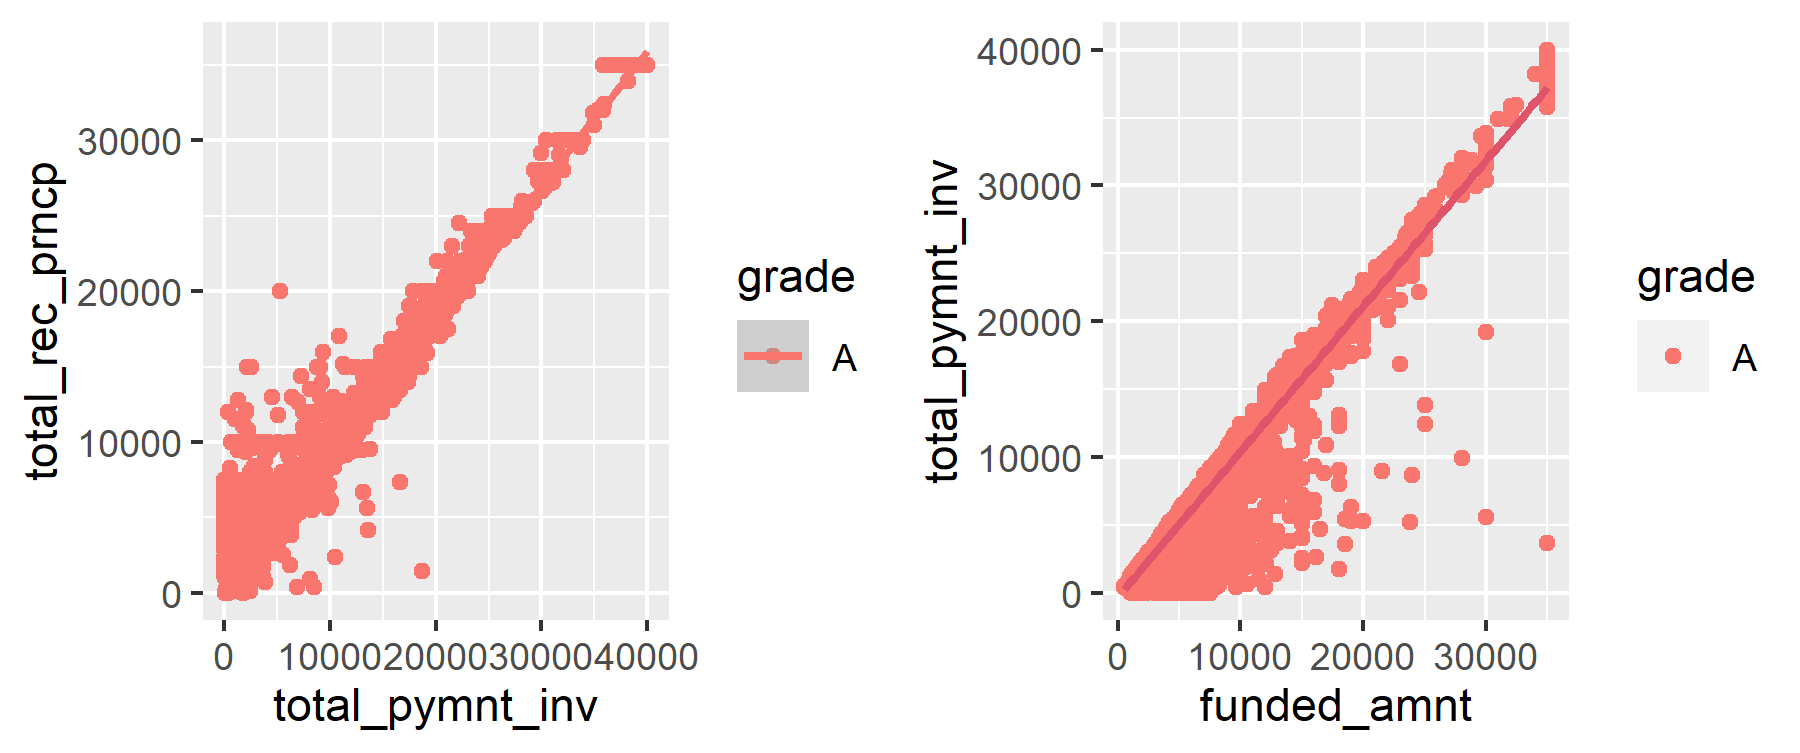
\includegraphics[scale=1.1]{imgs/scatter plot1.png}
\caption{Scatter plots sobre clientes con calificación crediticia A con errores}
    \label{fig3}
\end{figure}

\begin{figure}[H]
\centering
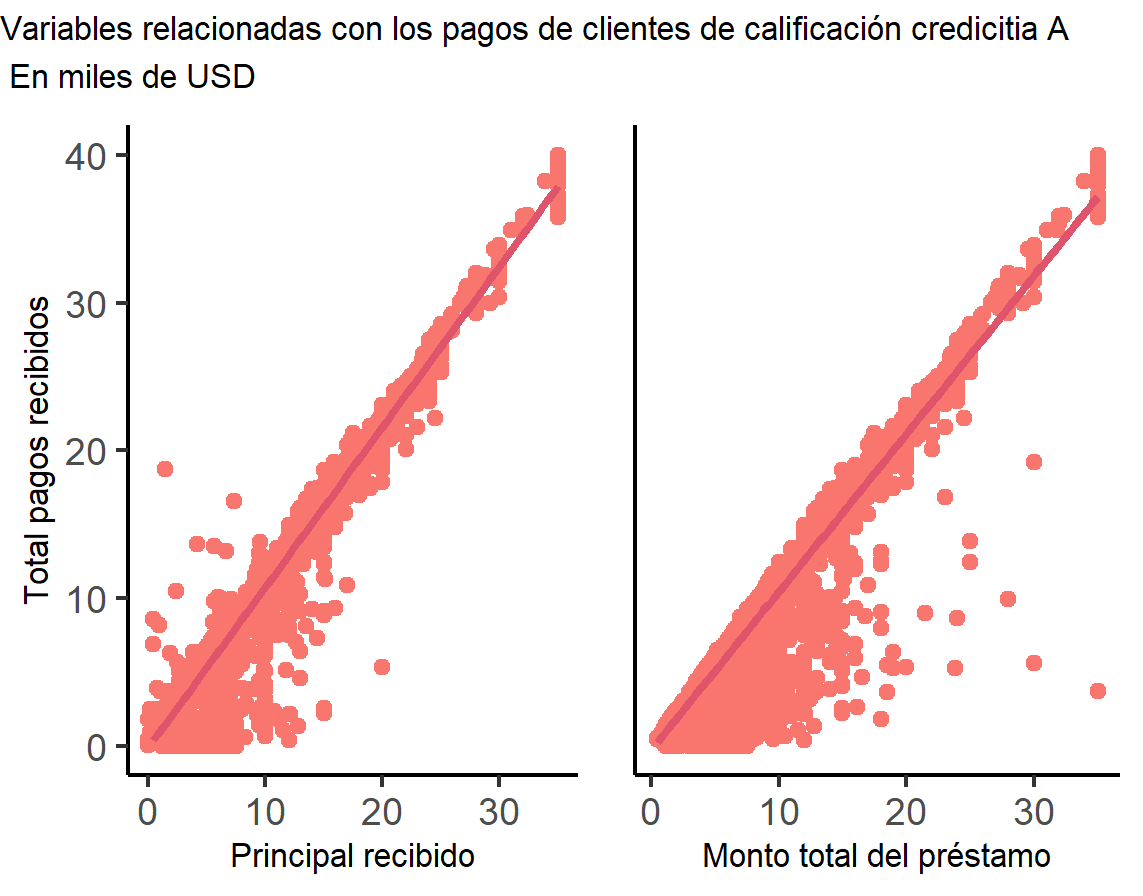
\includegraphics[scale=1.3]{imgs/scatter plot2.png}
\caption{Scatter plots sobre clientes con calificación crediticia A corregido}
    \label{fig4}
\end{figure}

\section*{Boxplots con datos de préstamos}
La Figura \ref{fig5} incumple con los 3 criterios. En primer lugar, al igual que en el caso anterior se presentan los títulos de los ejes con abreviaciones de los nombres de las variables que no son claros, se utilizan números de varias cifras que dificultan la lectura y además los valores del eje $x$ se superponen. En segundo lugar, siguiendo el principio 3, sería conveniente incluir el texto de la leyenda dentro del mismo gráfico. Si bien no es deseable que se repitan las calificaciones crediticias, teniendo en cuenta que el objetivo es comparar las distribuciones de acuerdo a la calificación crediticia y la propiedad de la vivienda del cliente, resulta más comprensible para poder comparar entre categorías armar sub-gráficos a partir de la titularidad de la vivienda como se muestran en la Figura \ref{fig5}. En este caso, se tiene en el eje $x$ a las distintas calificaciones y de esta forma es más sencillo comparar entre ellas.

\begin{figure}[H]
\centering
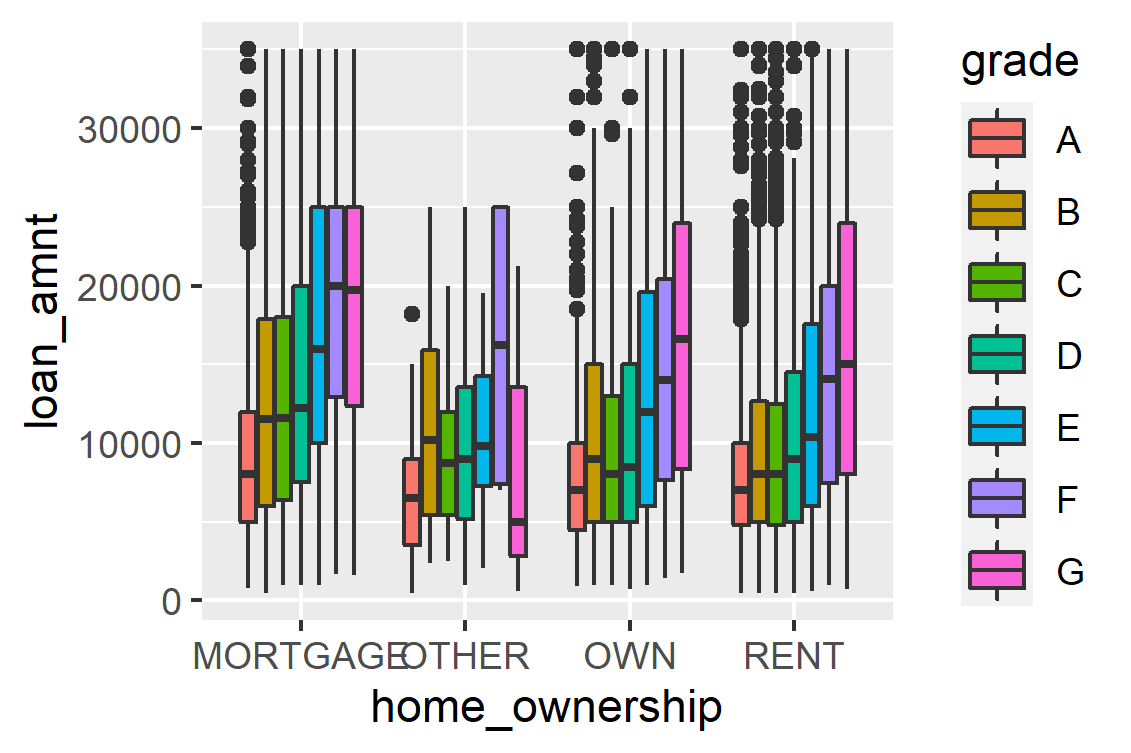
\includegraphics[scale=1.2]{imgs/loans1.png}
\caption{Boxplot con errores}
    \label{fig5}
\end{figure}

\begin{figure}[H]
\centering
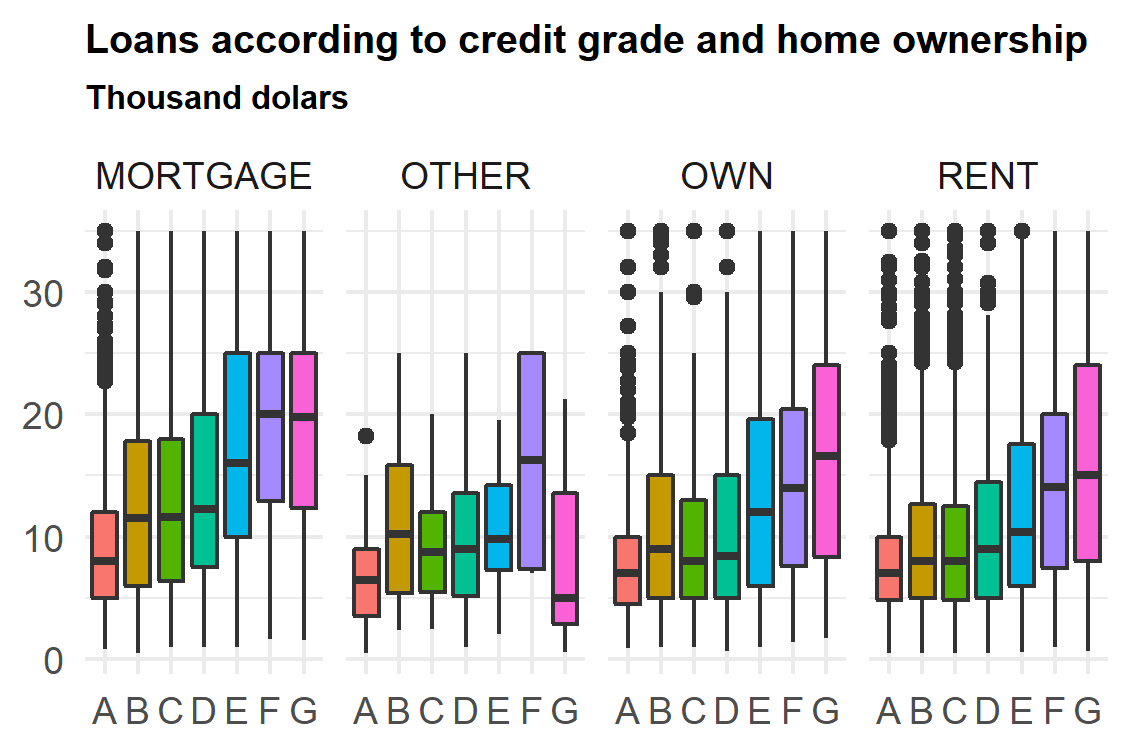
\includegraphics[scale=1.2]{imgs/loans2.png}
\caption{Boxplot corregido}
    \label{fig6}
\end{figure}

Por último, se presenta la Figura \ref{fig7} como nueva propuesta para comparar los niveles de préstamos según la calificación crediticia y la titularidad de la propiedad. Los gráficos no muestran exactamente lo mismo, ya que los boxplot muestran distribuciones de los préstamos condicionadas en las variables mencionadas mientras que la Figura 7 contiene el promedio. Sin embargo, si el objetivo es analizar los montos de préstamos otorgados para ver si se encuentran diferencias según la calificación crediticia y titularidad de la propiedad, puede resultar de interés analizar los promedios ya que aportan un mensaje más claro sobre las relaciones.
\begin{figure}[H]
\centering
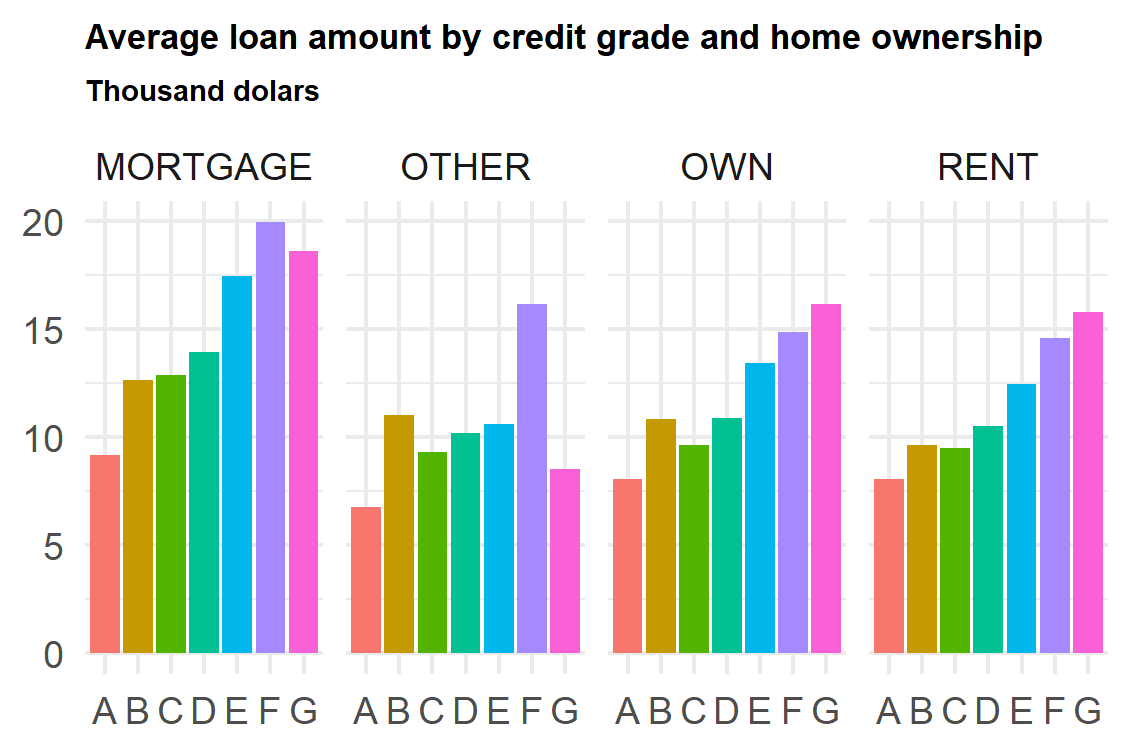
\includegraphics[scale=1.2]{imgs/loans3.png}
\caption{Nueva propuesta}
    \label{fig7}
\end{figure}


\end{document}